\chapter{Running on 16-bit hardware}
\label{chap:hardware}

%% CONTRIBUTION
{\small
\paragraph{Contributions} This chapter is largely based on the following publication\footnote{with the following author contributions.
Conceptualisation: MK, SH, MC. Data curation: MK. Formal Analysis: MK. Methodology: MK. Visualisation: MK. Writing – original draft:
MK. Writing – review \& editing: MK, SH, MC, PDD, TNP. The contributions of Sam, Matteo, Peter, and Tim are highly appreciated.}

\vspace{\baselineskip}
\indent M Klöwer, S Hatfield, M Croci, PD Düben and TN Palmer, 2021. \emph{Fluid simulations accelerated with 16 bit:
Approaching 4x speedup on A64FX by squeezing ShallowWaters.jl into Float16}, \textbf{Journal of Advances in Modeling
Earth Systems}, in review. Preprint \href{https://doi.org/10.1002/essoar.10507472.2}{10.1002/essoar.10507472.2}
\vspace{\baselineskip}}

\section{Introduction}

The first numerical weather prediction models have recently moved away from 64-bit double precision floating-point numbers
for higher computational efficiency in lower precision \citep{Govett2017,Nakano2018,Rudisuhli2013,Vana2017}. While both Float32
and Float64 formats are widely available for high-performance computing, support for 16-bit arithmetic is only available on mainstream
hardware for a few years, due to the demand for low precision by the deep learning community. The transition for an existing application
towards 16 bit is challenging: Rounding errors from low precision have to be controlled and a limited range of representable numbers
cannot be exceeded without causing often catastrophic under and overflows. But the potential performance gains are promising,
with 4x speedups compared to 64-bit calculations, not to mention the reduced energy consumption.

The current boom in machine learning applications is supported by advances in microprocessors. Instead of conventional central
processing units (CPU), graphic and tensor processing units GPU, TPU \citep{Jouppi2018,Jouppi2018a,Jouppi2017,Steinkraus2005}
are used, which are better suited for the workloads of machine learning. While most supercomputers are based on Intel CPUs with
the x86-64 architecture \citep{Dongarra2011}, many new installations transition towards GPUs or alternative microprocessor architectures
\citep{Zheng2020}. The trend is towards heterogeneous computing with specialised hardware, which is both a challenge and an
opportunity for weather and climate models \citep{Bauer2021,Bauer2021a}. Fugaku, the world’s fastest supercomputer as of 2020,
is based on Fujitsu’s A64FX processors with ARM architecture \citep{Odajima2020,Sato2020}. The A64FX also implements the
Float16 format (1 sign, 5 exponent and 10 mantissa bits) and Fujitsu promises a four-fold increase in the number of floating-point
operations per second. 

Float16 is the 16-bit variant of Float32 and Float64 and is defined in the 2008 revision of the IEEE-754 standard on floating-point arithmetic
\citep{IEEE1985,IEEE2008}. Alternatives such as bfloat16 \citep{Burgess2019, Kalamkar2019}, minifloats \citep{Fox2020}, logarithmic
fixed-point numbers \citep{Johnson2020,Johnson2018,Sun2020}, posits
\citep{Gustafson2017a,Chaurasiya2018,Klower2019a,Klower2020a,Langroudi2019,Zhang2020} and stochastic rounding
\citep{Croci2020,Hopkins2020,Mikaitis2020,Paxton2021} have been investigated, but most of these are not available on
standard supercomputing hardware. Currently only floats (and integers) enjoy a widely available support in terms of hardware,
libraries and compilers that ultimately make it possible to execute complex computational applications.

The use of low-precision number formats is motivated as in the presence of large uncertainties in the climate system rounding
errors are masked by other sources of error \citep{Palmer2015}. Typical rounding errors from high-precision calculations are
many orders of magnitude smaller than errors in the observations, from coarse resolution or underrepresented physical processes.
Low-precision calculations are therefore, at least in theory, sufficient without a loss in accuracy for a weather forecast or a climate prediction.
Emulated in parts of weather and climate models, 16-bit half precision has been shown to be a potential route to accelerated simulations
\citep{Dawson2018,Chantry2019, Hatfield2019, Klower2020a}.

Although weather and climate model data often comes with large uncertainties, many intermediate calculations inside a model simulation
require a higher precision. Time integration is often a precision-critical part of numerical simulations of dynamical systems. Stability constraints
require small time steps such that tendencies are often several times smaller than the prognostic variables \citep{Courant1967}.
Adding the two yields a loss of precision from the tendency as small increments can only be poorly resolved in low precision
\citep{Gill1951,Kahan1965,Moller1965}. In extreme cases this can lead to a model stagnation \citep{Croci2020}, and is often
dealt with using mixed-precision approaches \citep{Dawson2018,Klower2020a,TintoPrims2019}, where the tendencies are computed
in low-precision, but converted to a high-precision format before addition. This is beneficial as a large share of computing time is
accelerated with low precision, while precision-critical operations are kept in high precision.

Precision loss in calculations can be analysed with a variety of available tools, like FPBench \citep{Damouche2017},
CADNA \citep{Jezequel2008}, Verrou \citep{Fevotte2019}, and Verificarlo \citep{Denis2016}. Such tools are often either
based on interval arithmetic, providing rigid rounding error bounds, or on stochastic arithmetic to assess the rounding error growth.
While these can be useful to identify the minimal decimal precision for simulating chaotic systems, analysing the limited dynamic range
of low precision number formats is largely unaddressed in these tools.

Here, we present, to our knowledge, the first fluid circulation model that runs entirely in hardware-accelerated 16-bit floats on the
ARM architecture-based microprocessor A64FX. Strategies are presented to solve precision and range issues with 16-bit arithmetic:
In section \ref{sec:hardware_methods} we scale the shallow water equations, and an appropriate scale is found with the
newly-developed analysis-number format Sherlogs.jl. Additionally, a compensated time integration is presented to minimise
precision issues. Section \ref{sec:hardware_speedup} analyses the rounding errors of Float16 in ShallowWaters.jl and
benchmarks the performance compared to Float64. Section \ref{sec:hardware_discussion} discusses the results.

\begin{figure}[tbhp]
	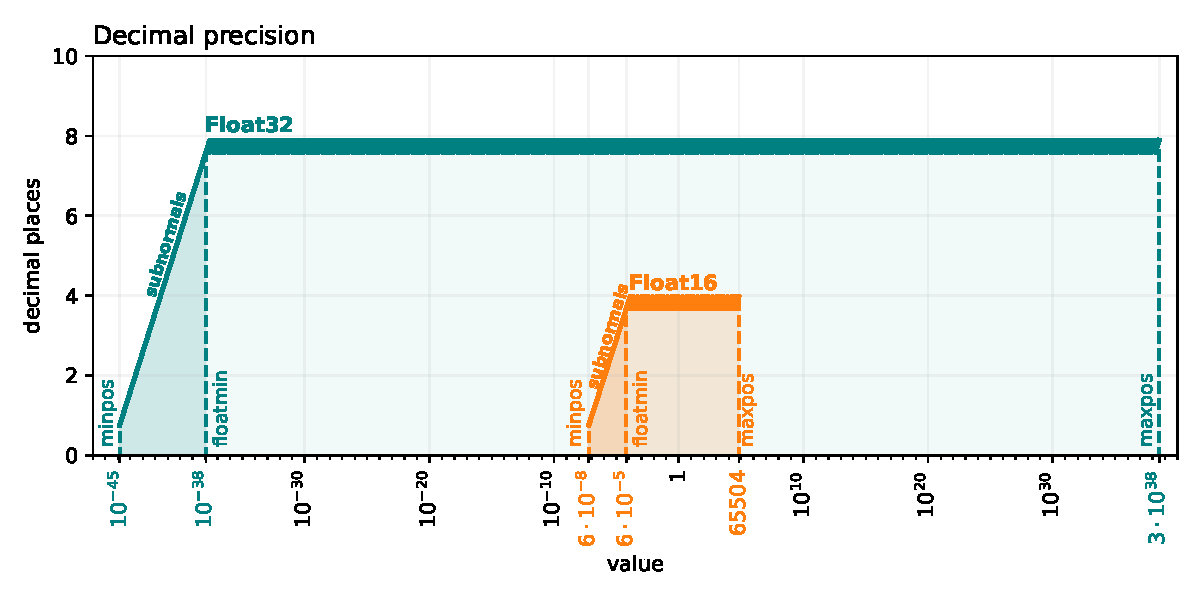
\includegraphics[width=1\textwidth]{Figures/a64fx/float32_16_decprec.pdf}
	\caption{\textbf{Decimal precision of Float16 and Float32 over the range of representable numbers.}
	The decimal precision is worst-case, i.e. given in terms of decimal places that are at least correct after rounding (see section \ref{}).
	The smallest representable number (minpos, see section \ref{}), the smallest normal number (floatmin) and the largest representable number
	(maxpos) are denoted with vertical dashed lines. The subnormal range is between minpos and floatmin.}
	\label{fig:a64fx_decprec}
\end{figure}

\section{Methods}
\label{sec:hardware_methods}

\subsection{Scaling the shallow water equations}
\label{sec:swm_scaling}

The shallow water equations describe atmospheric or oceanic flow idealised to two horizontal dimensions. They result from
a vertical integration of the Navier-Stokes equations \citep{Gill1982,Vallis2006} and are simplified but representative of many
weather and climate models, which are usually solved with many vertically-coupled horizontal layers. They describe the time
evolution of the prognostic variables velocity $\mathbf{u} = (u,v)$, and interface height $\eta$  in the following form 
\begin{align}
\partial_t\mathbf{u} &+ \mathbf{u} \cdot \nabla \mathbf{u} + f\mathbf{z} \times \mathbf{u} =
-g\nabla \eta + \nu_B \nabla^4 \mathbf{u} - r \mathbf{u} + \mathbf{F} \nonumber \\
\partial_t\eta &+ \nabla \cdot (\mathbf{u}h) = 0 \nonumber \\ 
\partial_tq &+ \mathbf{u} \cdot \nabla q = -\tau(q-q_0)
\end{align}
defined over a rectangular domain with zonal and meridional coordinates $x,y$ of size $L_x = 8000\op{km}$,
$L_y  = 4000\op{km}$, respectively. The domain is a zonal channel with boundary conditions being periodic in $x$.
The channel setup is motivated by zonal flows like the Antarctic Circumpolar Current but highly idealised \citep{Jansen2015,Jansen2015a}.

The non-linear momentum advection is $\mathbf{u} \cdot \nabla\mathbf{u}$. The Coriolis force is
$f\hat{z} \times \mathbf{u} = (-fv,fu)$ with the Coriolis parameter $f$ using a $\beta$-plane approximation at 45\textdegree{}N.
The pressure gradient $-g\nabla \eta$ scales with a reduced gravitational acceleration $g = 0.01\op{ms}^{-2}$ to represent
baroclinic ocean/atmosphere dynamics \citep{Gill1982}. The zonal wind forcing $\mathbf{F} = (F_x,0)$ is a meridional shear
$F_x = F_0\sin(\omega t) \tanh(2\pi(L_y^{-1} - \tfrac{1}{2}))$ which reverses seasonally ($\omega^{-1} = 365\op{days}$).
Lateral diffusion of momentum is described by $\nu_B\nabla^4\mathbf{u}$, with biharmonic viscosity coefficient $\nu_B$.
Linear bottom friction is represented by $-r\mathbf{u}$ which decelerates the flow at a time scale of $r^{-1} = 300\op{days}$.
The equation for interface height $\eta$ is the shallow water-variant of the continuity equation, ensuring conservation of volume
(and mass as the density $\rho$ is constant). The layer thickness is $h = \eta + H$ of a fluid with depth $H$ at rest.
Several meridional ridges on the seafloor trigger instabilities in the zonal flow, but they are small compared to the fluid depth.
The shallow water equations are complemented with an advection for the passive tracer $q$ , which is stirred by the flow
through $\mathbf{u} \cdot \nabla q$ and slowly ($\tau^{-1} = 100\op{days}$) relaxed back to a reference $q_0$.

In order to control the range of numbers occurring in the simulation, the shallow water equations are scaled with a multiplicative
constant. The evaluation of linear terms is not affected, but the non-linear terms involve an unscaling. The same constant $s$
is chosen for zonal velocity $u$  and meridional velocity $v$, such that $\hat{u} = su$ and $\hat{v} = sv$.
Additionally, we use dimensionless spatial gradients $\hat{\partial_x} = \Delta x \partial_x, \hat{\nabla} = \Delta x \nabla$, etc.
by scaling the equations with the grid spacing $\Delta x$. For simplicity, we use the same $\Delta x$ in $x$ and $y$-direction
but generalisation to less regular grids is possible. The grid spacing $\Delta x$ is then combined with the time step
$\widehat{\Delta t} = \tfrac{\Delta t}{\Delta x}$ and $\hat{\partial_t} = \Delta x \partial_t$. Due to the 4th-order gradient in the
viscosity, we scale its coefficient as $\hat{\nu_B} = \Delta x^{-3}\nu_B$. Using the potential vorticity $h^{-1}(f + \zeta)$,
with the relative vorticity $\zeta = \partial_xv - \partial_yu$, and the Bernoulli potential $\tfrac{1}{2}(u^2 + v^2) + g\eta$,
the shallow water equations can be written into a scaled form as

\begin{align}
\hat{\partial_t}\hat{u} &= \frac{[s\Delta x f]+ \hat{\zeta}}{\hat{h}}\frac{\hat{v}\hat{h}}{s} -\hat{\partial_x}
\left([\frac{1}{2s}](\hat{u}^2 + \hat{v}^2) + [\frac{sg}{s_\eta}]\hat{\eta} \right) + \hat{\nu_B} \hat{\nabla}^4 \hat{u}
- [r\Delta x]\hat{u} + [s\Delta x F_x] \nonumber \\
\hat{\partial_t}\hat{v} &= - \frac{[s\Delta x f]+ \hat{\zeta}}{\hat{h}}\frac{\hat{u}\hat{h}}{s} -\hat{\partial_y}
\left([\frac{1}{2s}](\hat{u}^2 + \hat{v}^2) + [\frac{sg}{s_\eta}]\hat{\eta} \right) + \hat{\nu_B} \hat{\nabla}^4 \hat{v}
- [r\Delta x]\hat{v} + [s\Delta x F_y]
\end{align}
Square brackets denote pre-computed constants and only the volume fluxes $uh,vh$ have to be unscaled on every time step.
As the volume fluxes are quadratic terms, the evaluation of $\hat{u}\hat{h}$ scales as $s^2$, which therefore has to be
partly unscaled with $s^{-1}$. The continuity equation is rescaled with $s_\eta$, i.e. $\hat{\eta} = s_\eta \eta$ as well as
$\hat{h} = \hat{\eta} + s_\eta H$, and the tracer advection equation is rescaled with $s_q$, so that $\hat{q} = s_q q$
\begin{align}
\hat{\partial_t} \hat{\eta} &= -\hat{\partial_x}(\frac{\hat{u}\hat{h}}{s}) - \hat{\partial_y}(\frac{\hat{v}\hat{h}}{s}) \nonumber \\
[s\hat{\partial_t}] \hat{q} &= \left(-\hat{u}\hat{\partial_x} \hat{q} - \hat{v}\hat{\partial_y} \hat{q}\right) - [\tau \Delta x](\hat{q} - \hat{q_0})
\end{align}

ShallowWaters.jl solves these scaled shallow water equations with 2nd order finite differencing on a regular,
but staggered Arakawa C-grid \citep{Arakawa1977}. The advection of potential vorticity uses the energy
and enstrophy-conserving scheme of \cite{Arakawa1990}. The tracer advection equation for $q$ is solved
with a semi-Lagrangian advection scheme \citep{Diamantakis2013,Smolarkiewicz1992}. This scheme calculates
a departure point for every arrival grid point one time step ago. The tracer field is then interpolated onto the departure point,
which is used as the tracer concentration at the arrival point for the next time step. More details on the implementation of
the semi-Lagrangian advection scheme is described in \citep{Klower2020a}. The time integration of ShallowWaters.jl is
discussed in section \ref{sec:compensated_time_integration}.

\subsection{Choosing a scale with Sherlogs}
\label{sec:scale_sherlogs}

The scaling of equations has to be implemented carefully when using number formats with a limited dynamic range,
such as Float16 (Fig. \ref{fig:a64fx_decprec}). Subnormals for Float16 are in the range of $6 \cdot 10^{-8}$ to
$6 \cdot 10^{-5}$ (see section \ref{}) and are inefficiently supported on some hardware, such that their occurrence
causes large performance penalties. This reduces the available range of Float16 even further and a simulation
has to fit as best as possible in the remaining 9 orders of magnitude between $6.104 \cdot 10^{-5}$ and $65504$.
A single overflow, i.e. a result above $65504$, will abort the simulation. Understanding the range of numbers
that occur in all operations and ideally in which lines of the code is therefore very important. 
For most algorithms this is very difficult to achieve unless the numbers are directly measured within the simulation. 

\begin{figure}[tbhp]
\begin{lstlisting}[language=JuliaLocal, label=lst:sherlogs, caption={\textbf{Example usage and output of Sherlogs.jl,
a package for Sherlogs and DrWatson, two analysis-number formats that can be combined with type-flexible
functions in Julia.} Using Sherlog16 as the first argument of \texttt{run\_model} runs ShallowWaters.jl with Float16 but
also logs the bitpattern of every arithmetic result into a \emph{logbook} of length $2^{16}=65536$ to create a bitpattern
histogram. \texttt{DrWatson16\{f\}} uses Float16 but also records a stack trace (a list of calling functions and respective
lines of code) every time the function \texttt{f(x)} evaluates to \texttt{true} with the arithmetic result \texttt{x}.
Here, a subnormal arises in a multiplication ($*$ in line 14 here) in line 320 of the code in script \texttt{time\_integration.jl.}}]
julia> using ShallowWaters, Sherlogs       # load packages
julia> # run ShallowWaters with Sherlog16 which logs all arithmetic results
julia> run_model(Sherlog16)                # use Sherlog16 as number format

julia> get_logbook()                       # retrieve the bitpattern histogram
65536-element LogBook(1112720887, 1484631, 1378491, 1024411, ... , 0, 0, 0)

julia> # run ShallowWaters with DrWatson16 recording a stack trace when f=true
julia> f(x) = 0 < abs(x) < floatmin(Float16)  # true for subnormals
julia> run_model(DrWatson16{f})            # use DrWatson16 as number format

julia> get_stacktrace(1)                   # retrieve the first stack trace
3-element Vector{Base.StackTraces.StackFrame}:
* at DrWatson16.jl:52 [inlined]            # subnormal occurred in *
caxb!(...) at time_integration.jl:320      # inside this function
time_integration(...) at time_integration.jl:82 # called from here
\end{lstlisting}
\end{figure}

We therefore developed the analysis-number format Sherlogs. Sherlog16, for example, uses Float16 to compute,
but after every arithmetic operation the result is also logged into a bitpattern histogram. Running a simulation with
Sherlogs will take considerably longer due to the overhead from logging the arithmetic results, which can be obtained
in the form of a bitpattern histogram upon completion. The bitpattern histogram will reveal information such as the
smallest and largest occurring numbers or how well an algorithm fits into a smaller dynamic range.
An example usage of Sherlogs is given in Listing \ref{lst:sherlogs}.

Sherlogs are implemented in the package Sherlogs.jl, which makes use of the type-flexible
programming paradigm in Julia \citep{Bezanson2017}. A function is written in an abstract form,
which is then dynamically dispatched to the number format provided and compiled just-in-time.
Such a number format can therefore be, for example, Float64 or Float16, but also any user-defined
number format such as Sherlogs.

An appropriate scaling $s,s_\eta,s_q$ has to be chosen for a given set of parameters. The bitpattern
histogram of the entirely unscaled shallow water equations simulated with Float32 reveals range issues
that would arise with Float16 (Fig. \ref{fig:a64fx_bitpatternhist}a). A large share (10\%) of the arithmetic
results would be below the representable range of Float16. Consequently, running the model without
any scaling modifications in Float16 would round many numbers to 0, causing so-called underflows
that deteriorate the simulated dynamics \citep{Klower2020a}. Most of these underflows occur in the
calculation of gradients, which consequently have to be non-dimensionalised as previously suggested
\citep{Klower2019a}. This also largely removes a resolution-dependence of the bitpattern histograms,
such that Float16 simulations are possible across a wide range of resolutions. Dimensionless gradients
are a major improvement to fit ShallowWaters.jl into the available range with Float16, yet 3\% of the
arithmetic results are subnormals (Fig. \ref{fig:a64fx_bitpatternhist}b). On A64FX a flag can be set to
avoid the performance penalty from subnormals by flushing every occurring subnormal to zero.
The smallest representable number is therefore $6.104 \cdot 10^{-5}$.

\begin{figure}[tbhp]
	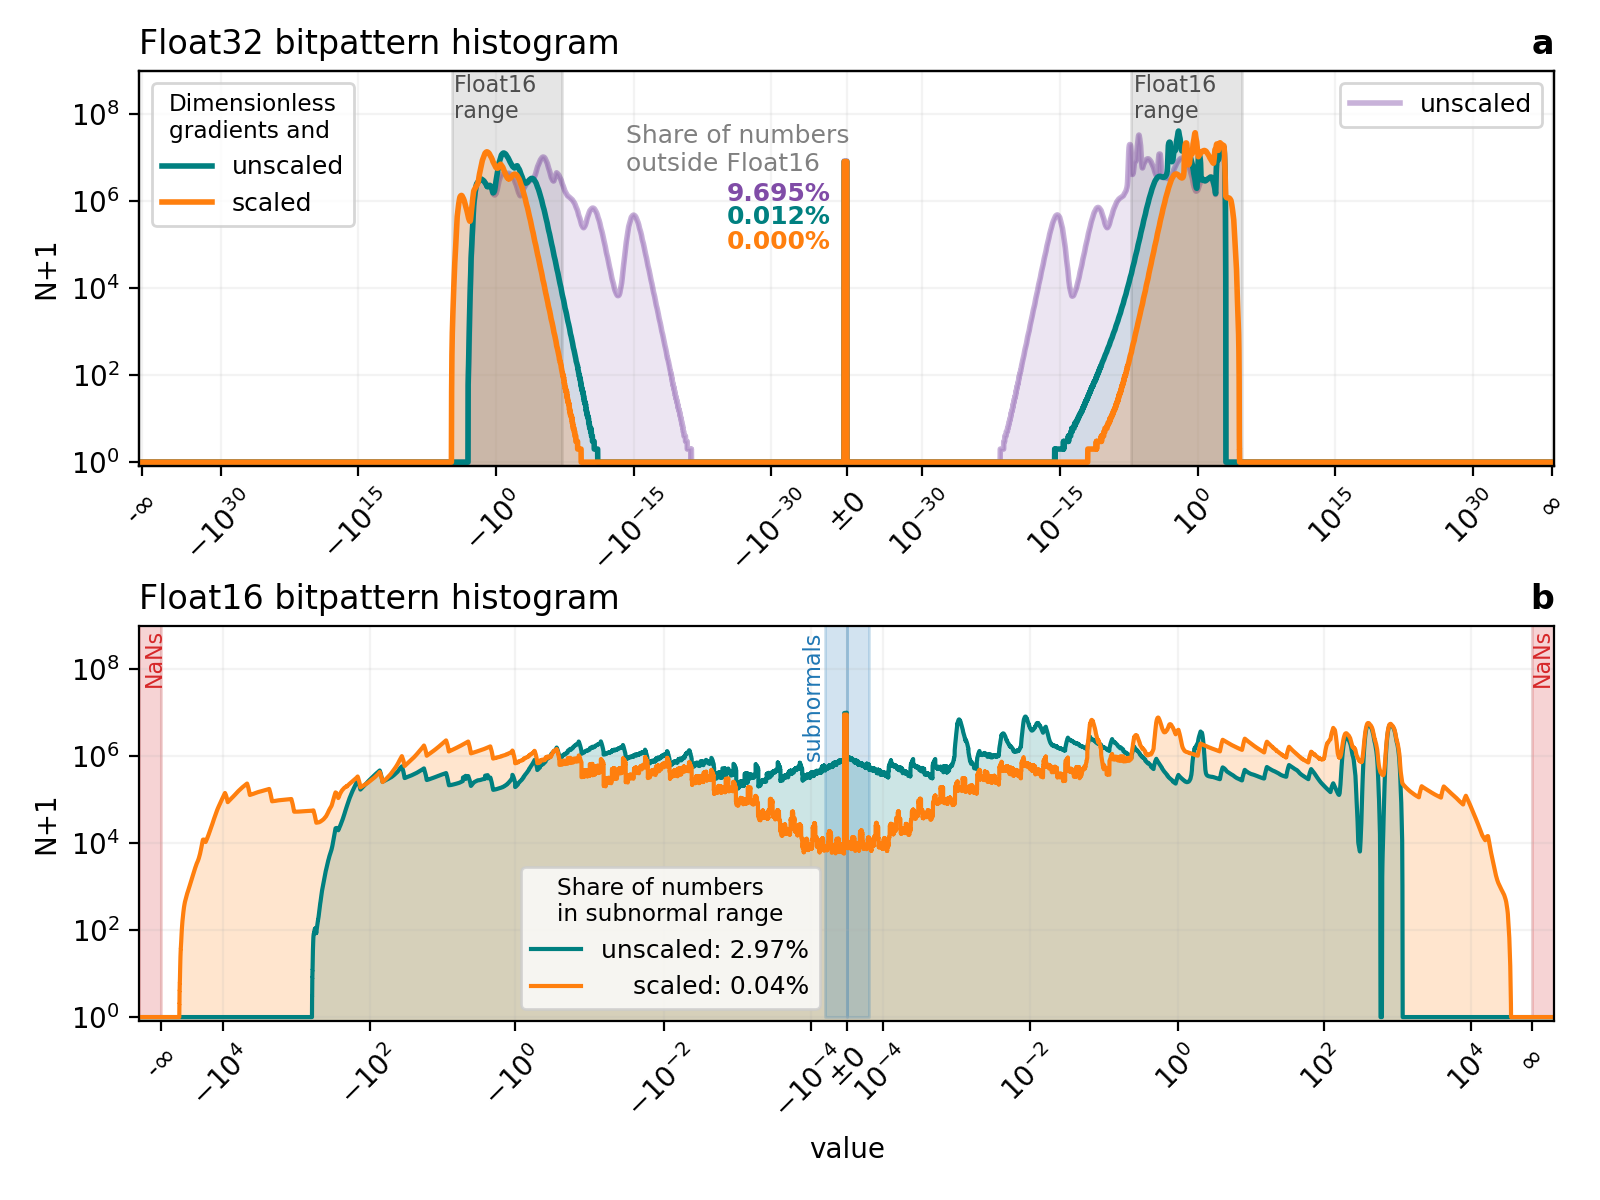
\includegraphics[width=1\textwidth]{Figures/a64fx/bitpattern_hist.png}
	\caption{\textbf{Bitpattern histogram of all arithmetic results in ShallowWaters.jl. a}
	200-day simulation at $\Delta x = 20\op{km}$ based on Float32 arithmetic. The share of numbers
	outside the Float16 range (grey shading) are colour-coded to the respective histograms. \textbf{b} as \textbf{a}
	but based on Float16. Bitpattern histograms are created with Sherlogs.jl. The logarithmic y-axis denotes the
	number of occurrences $N$ of the respective bitpattern during the simulation. The histograms span all
	available bitpatterns (\texttt{0x0000} to \texttt{0xffff} in hexadecimal) in the respective formats evenly
	but are sorted and relabelled with the corresponding values for readability. The range of bitpatterns that
	are subnormals or interpreted as Not-A-Number (NaN) are marked. Bitpatterns histograms are without
	compensated time integration.}
	\label{fig:a64fx_bitpatternhist}
\end{figure}

Using the DrWatson number format from Sherlogs.jl identifies the addition of the tendencies to the
prognostic variables $u,v,\eta$ as prone to produce subnormals (Listing \ref{lst:sherlogs}). We therefore
increase the scales  to scale up the prognostic variables and consequently their tendencies. Choosing
$s = s^6, s_\eta = 1$ reduces the amount of subnormals to 0.04\%, while leaving about a factor two
headspace between the largest occurring numbers (about $30000$) to avoid overflows beyond $65504$
(Fig. \ref{fig:a64fx_bitpatternhist}b). The compensated time integration (see section
\ref{sec:compensated_time_integration}) increases this share to about 0.2\%.

The idealised tracer in ShallowWaters.jl takes values in (-1,1), so we scale this variable by $s_q = 2^{15}$
in order to use most of the Float16 range. This is to allow as many bitpatterns as possible for the interpolation
in the semi-Lagrangian advection scheme, which uses non-dimensional departure points on a locally relative
grid for 16-bit arithmetic, as described in \cite{Klower2020a}.

Consequently, the fully scaled shallow water equations are squeezed well into Float16, making near-optimal
use of the available bitpatterns, of which only 3\% are unused (NaNs excluded). In contrast, a simulation with
Float32 does not make use of at least 81\% of available bitpatterns (Fig. \ref{fig:a64fx_bitpatternhist}), assuming
that for a simulation run long enough all bitpatterns within the used range occur eventually. Extrapolating this
to Float64 with a representable range of $5 \cdot 10^{-324}$ to $2 \cdot 10^{308}$ the share of unused bitpatterns
is at least 97.5\%. This computational inefficiency can be overcome with 16-bit number formats and systematic
scaling as presented here. However, scaling leaves the precision issues with low-precision formats unaddressed,
for which we present a technique in the next section.

\subsection{A compensated time integration}
\label{sec:compensated_time_integration}

To minimize the precision loss in the time-integration, we adopt compensated summation as an alternative approach
to mixing precision. Compensated summation is a simple, yet powerful technique that prevents the accumulation of
rounding errors in the computation of large sums. Since the addition of multiple terms is ubiquitous in scientific computing,
compensated summation can be used to improve the accuracy of many algorithms such as numerical linear algebra
operations, integration or optimisation. Here we use compensated summation to augment the resilience to rounding
errors of our half-precision time-stepping method. 

The first version of compensated summation was used by \cite{Gill1951} in a Runge-Kutta integrator scheme in
fixed-point arithmetic, and the idea was subsequently extended to floating-point arithmetic by \cite{Kahan1965},
\cite{Moller1965} and others \citep{Vitasek1969,Linnainmaa1974,Higham1993}. That we are aware of, our paper
is the first work in which compensated summation is used in a fluid circulation model with 16-bit arithmetic.

To understand compensated summation, consider the following naïve algorithm for the summation of all the
entries of a length-$n$ vector $a$ with elements $a_i, i = 1,...,n$

\begin{lstlisting}[language=JuliaLocal]
sum = 0             # variable to store the sum
for ai in a         # loop over all elements of a
	sum += ai       # accumulate each element into sum   
end
return sum
\end{lstlisting}

This algorithm is prone to rounding errors, which accumulate at a rate proportional to $n$ \citep{Higham1993}.
Furthermore, the algorithm might cause stagnation, a phenomenon for which the partial sum becomes too large,
causing each subsequent addition to be neglected due to rounding. Compensated summation offers a much
better alternative at the cost of introducing an additional compensation variable \texttt{c}:

\begin{lstlisting}[language=JuliaLocal]
c = 0                      # compensation, initially 0
sum = 0                    # variable to store the sum
for ai in a                # loop over all elements of a
	aic = ai - c           # compensate rounding error from previous iteration
 	temp = sum + aic       # add next element of a, but store in temp
	c = (temp-sum) - aic   # rounding error from sum+aic
 	sum = temp             # copy addition back to sum
end
return sum
\end{lstlisting}

At infinite precision, the compensation \texttt{c} will remain 0. At finite precision, however, calculating \texttt{c = (temp-sum) - aic}
will estimate the rounding error in the addition \texttt{sum + aic} and subsequently attempt to compensate for it in the next iteration
through \texttt{aic = ai - c}. For base-2 floating point arithmetic we have exactly \texttt{sum + ai = temp + c}, i.e. the compensation
variable \texttt{c} correctly captures the rounding errors in the addition. Compensated summation prevents the rounding errors
from accumulating, and the overall summation error will stay a mere multiple of machine precision \citep{Higham1993}. Overall,
the compensation \texttt{c} can be interpreted as a storage variable for rounding errors and effectively prevents rounding errors
in the summation from growing beyond machine precision accuracy.

Compensated summation is especially useful in settings in which the order of summation cannot be manipulated to prevent
rounding error growth. Time integration schemes, for which the state variables are updated sequentially, are especially
amenable to augmentation by compensated summation. Over a time period $T$ the number of terms to be added scales
as $T\Delta t^{-1}$, proportional to one for each time step. The naÏve algorithm would cause rounding errors to grow like
$\mathcal{O}(T\Delta t^{-1}\varepsilon)$, causing errors to counter-intuitively grow as the time-step is refined.
With compensated summation the rounding errors will stay $\mathcal{O}(\varepsilon)$.

ShallowWaters.jl uses the 4th-order Runge-Kutta scheme \citep{Butcher2008} to integrate the non-dissipative terms in time:
The momentum advection $\mathbf{u} \cdot \nabla \mathbf{u}$;
the Coriolis force $f\hat{z} \times \mathbf{u}$;
the pressure gradient $-g\nabla \eta$;
the wind forcing $\mathbf{F}$;
and the conservation of volume $-\nabla \cdot (\mathbf{u} h)$ are summarised as the right-hand side function $\op{rhs}$.
The time integration is now augmented with compensated summation. The rounding error $c_u$ that occurs in the addition
of the total tendency $du$ to the previous time step $u_n$ is calculated and stored. On the next time step, this rounding error
is subtracted from the total tendency $du$ in an attempt to compensate for the rounding error from the previous time step.
This is illustrated here for the zonal velocity $u$ in isolation, although in practice the time integration has to update the
prognostic variables $u,v,\eta$ simultaneously. A compensated time integration for $u$ with RK4 can be written as
\begin{align}
k_1 &= \op{rhs}(u + \tfrac{\Delta t}{2}k_1) \nonumber \\
k_2 &= \op{rhs}(u + \tfrac{\Delta t}{2}k_2) \nonumber \\
k_3 &= \op{rhs}(u + \tfrac{\Delta t}{2}k_3) \nonumber \\
k_4 &= \op{rhs}(u + \Delta t k_3) \nonumber \\
du &= \tfrac{\Delta t}{6}(k_1 + 2k_2 + 2k_3 + k_4) \nonumber \\
u_{n+1}^* &= u_n + du \nonumber \\
c_u &= (u^*_{n+1} - u_n) - du
\label{eq:RK4_compensated}
\end{align}
with $c_u = 0$ as initial condition. The addition $u_n + du$ usually suffers from rounding errors as described above.
The loss of precision in $du$ is calculated in $c_u$ (which is only 0 in exact arithmetic). The compensation is analogously
implemented with $c_v,c_\eta$  for the other prognostic variables.  

The dissipative terms, i.e. biharmonic diffusion of momentum $\nu_B\nabla^4\mathbf{u}$ and bottom friction $-r\mathbf{u}$,
are integrated with a single forward step after the Runge-Kutta integration in ShallowWaters.jl and summarized as 
$\op{rhs}_{\op{diss}}$. To compensate for rounding errors for both the dissipative and non-dissipative terms simultaneously,
$c_u$ from Eq. \ref{eq:RK4_compensated} is subtracted from the total dissipative tendency $du_{\op{diss}}$.
In that sense, the rounding error from Eq. \ref{eq:RK4_compensated} is attempted to be compensated subsequently
in Eq. \ref{eq:RK4_compensated2}, and vice versa.
\begin{align}
du_{\op{diss}} &= \Delta t \op{rhs}_{\op{diss}}(u_{n+1}^*) - c_u \nonumber \\
u_{n+1} &= u^*_{n+1} + du_{\op{diss}} \nonumber \\
c_u &= (u_{n+1} - u_{n+1}^*) - du_{\op{diss}}
\label{eq:RK4_compensated2}
\end{align}
Only the addition of the total tendency is compensated here to minimise the amount of additional calculations, which
increases when also compensating the 3 sub steps in RK4.

The compensated time integration is an alternative to mixed-precision approaches. While those aim to keep the precision
high in the precision-critical calculations, the compensated time integration introduces a new variable to compensate for
the rounding errors in one precision-critical calculation. With compensated time integration all variables can be kept in 16 bit,
and no conversions between number formats are necessary.

\begin{figure}[tbhp]
	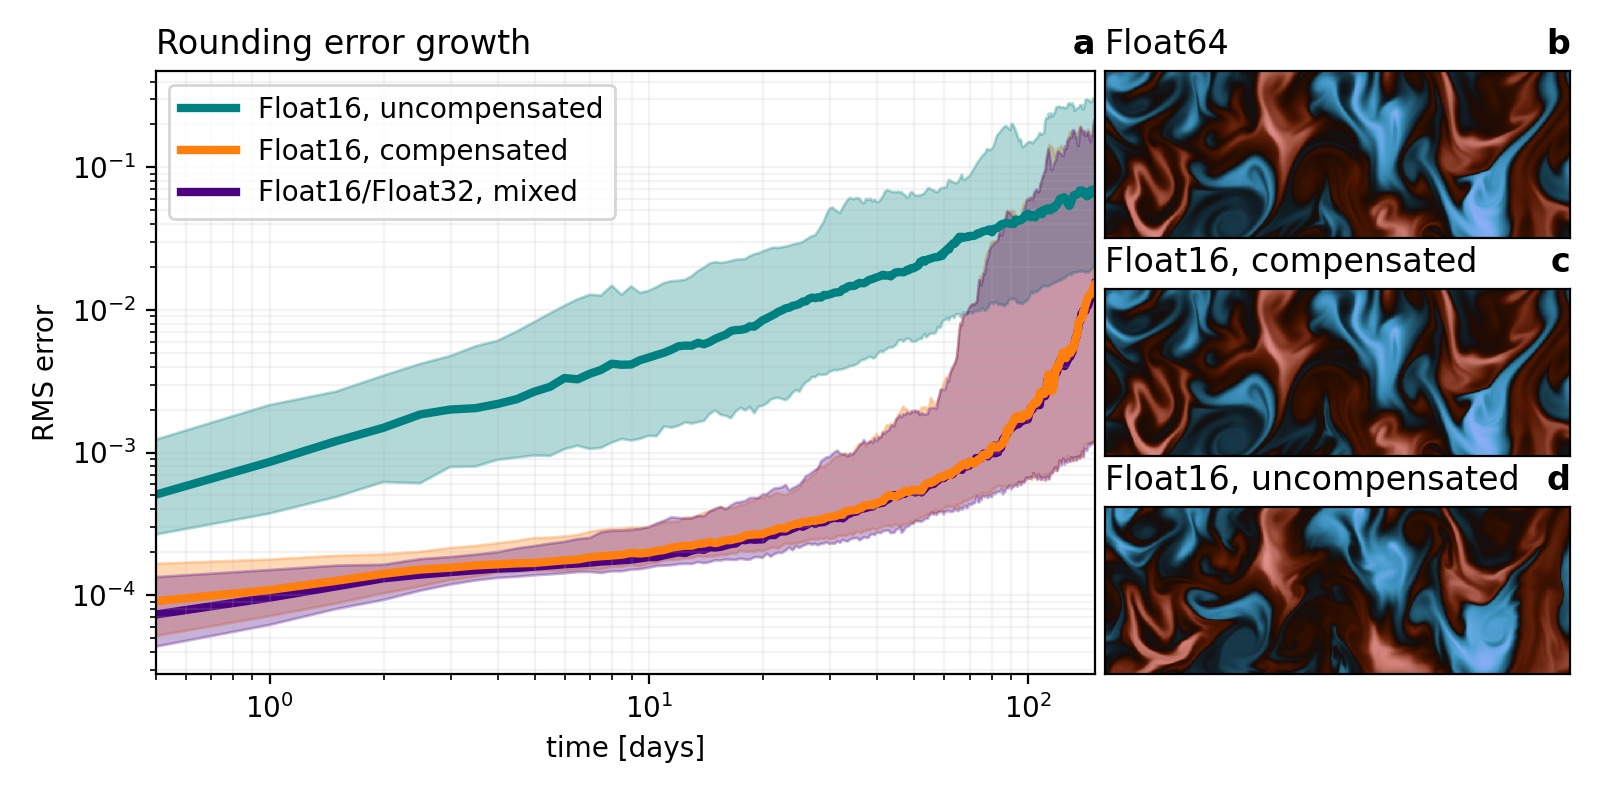
\includegraphics[width=1\textwidth]{Figures/a64fx/error_growth.png}
	\caption{\textbf{Rounding error growth with Float16 in ShallowWaters.jl
	using compensated time integration or mixed-precision. a}
	Errors are root-mean square (RMS) errors of zonal velocity $u$ relative to Float64. Solid lines denote the median
	and shadings the interdecile confidence interval. \textbf{b,c} Snapshots of tracer $q$ from a zoom into
	Fig. \ref{fig:a64fx_tracermixing} after 100 days of simulation and \textbf{d} as \textbf{c} but without
	compensated time integration.}
	\label{fig:a64fx_error_growth}
\end{figure}

\section{Results}
\label{sec:hardware_speedup}

\subsection{Minimizing precision issues in 16 bit}
The accumulated rounding error from mixing precision and compensated time integration is now assessed.
ShallowWaters.jl is started from identical, in Float16 perfectly representable, initial conditions in a domain of
8000~km by 4000~km. The model is spun-up to reach a turbulent flow domain-wide, while the tracer starts from
an idealised checkerboard pattern to better highlight the turbulence everywhere in the domain.  The grid consists
of 3000x1500 points at about 2.7~km grid-spacing. With Float16 and without compensated time integration,
the accumulated rounding error for zonal velocity $u$ compared to Float64 exponentially increases 100-fold in
the first 150 days (Fig. \ref{fig:a64fx_error_growth}a). With mixed-precision, using Float16 for the tendencies
and Float32 for the prognostic variables, this rounding error growth is strongly reduced. Errors after a few time steps
without mixed-precision are reached after about 100 days (about 25,000 time steps) of integration. After
that the error growth accelerates and chaos removes the information of the initial conditions.

Using a compensated time integration, the rounding error from Float16 is strongly reduced and matches well with the
error growth of mixed-precision. From the perspective of rounding errors the two methods are therefore equivalently
suited to reduce rounding errors with 16-bit arithmetic. The rounding error growth of the other prognostic variables is
similar. The positive effect of compensated time integration is well illustrated in snapshots of tracer mixing where even
after 100 days of simulation only a very slight deviation from the Float64 reference is observable
(Fig. \ref{fig:a64fx_error_growth}b, c and d).

\begin{figure}[tbhp]
	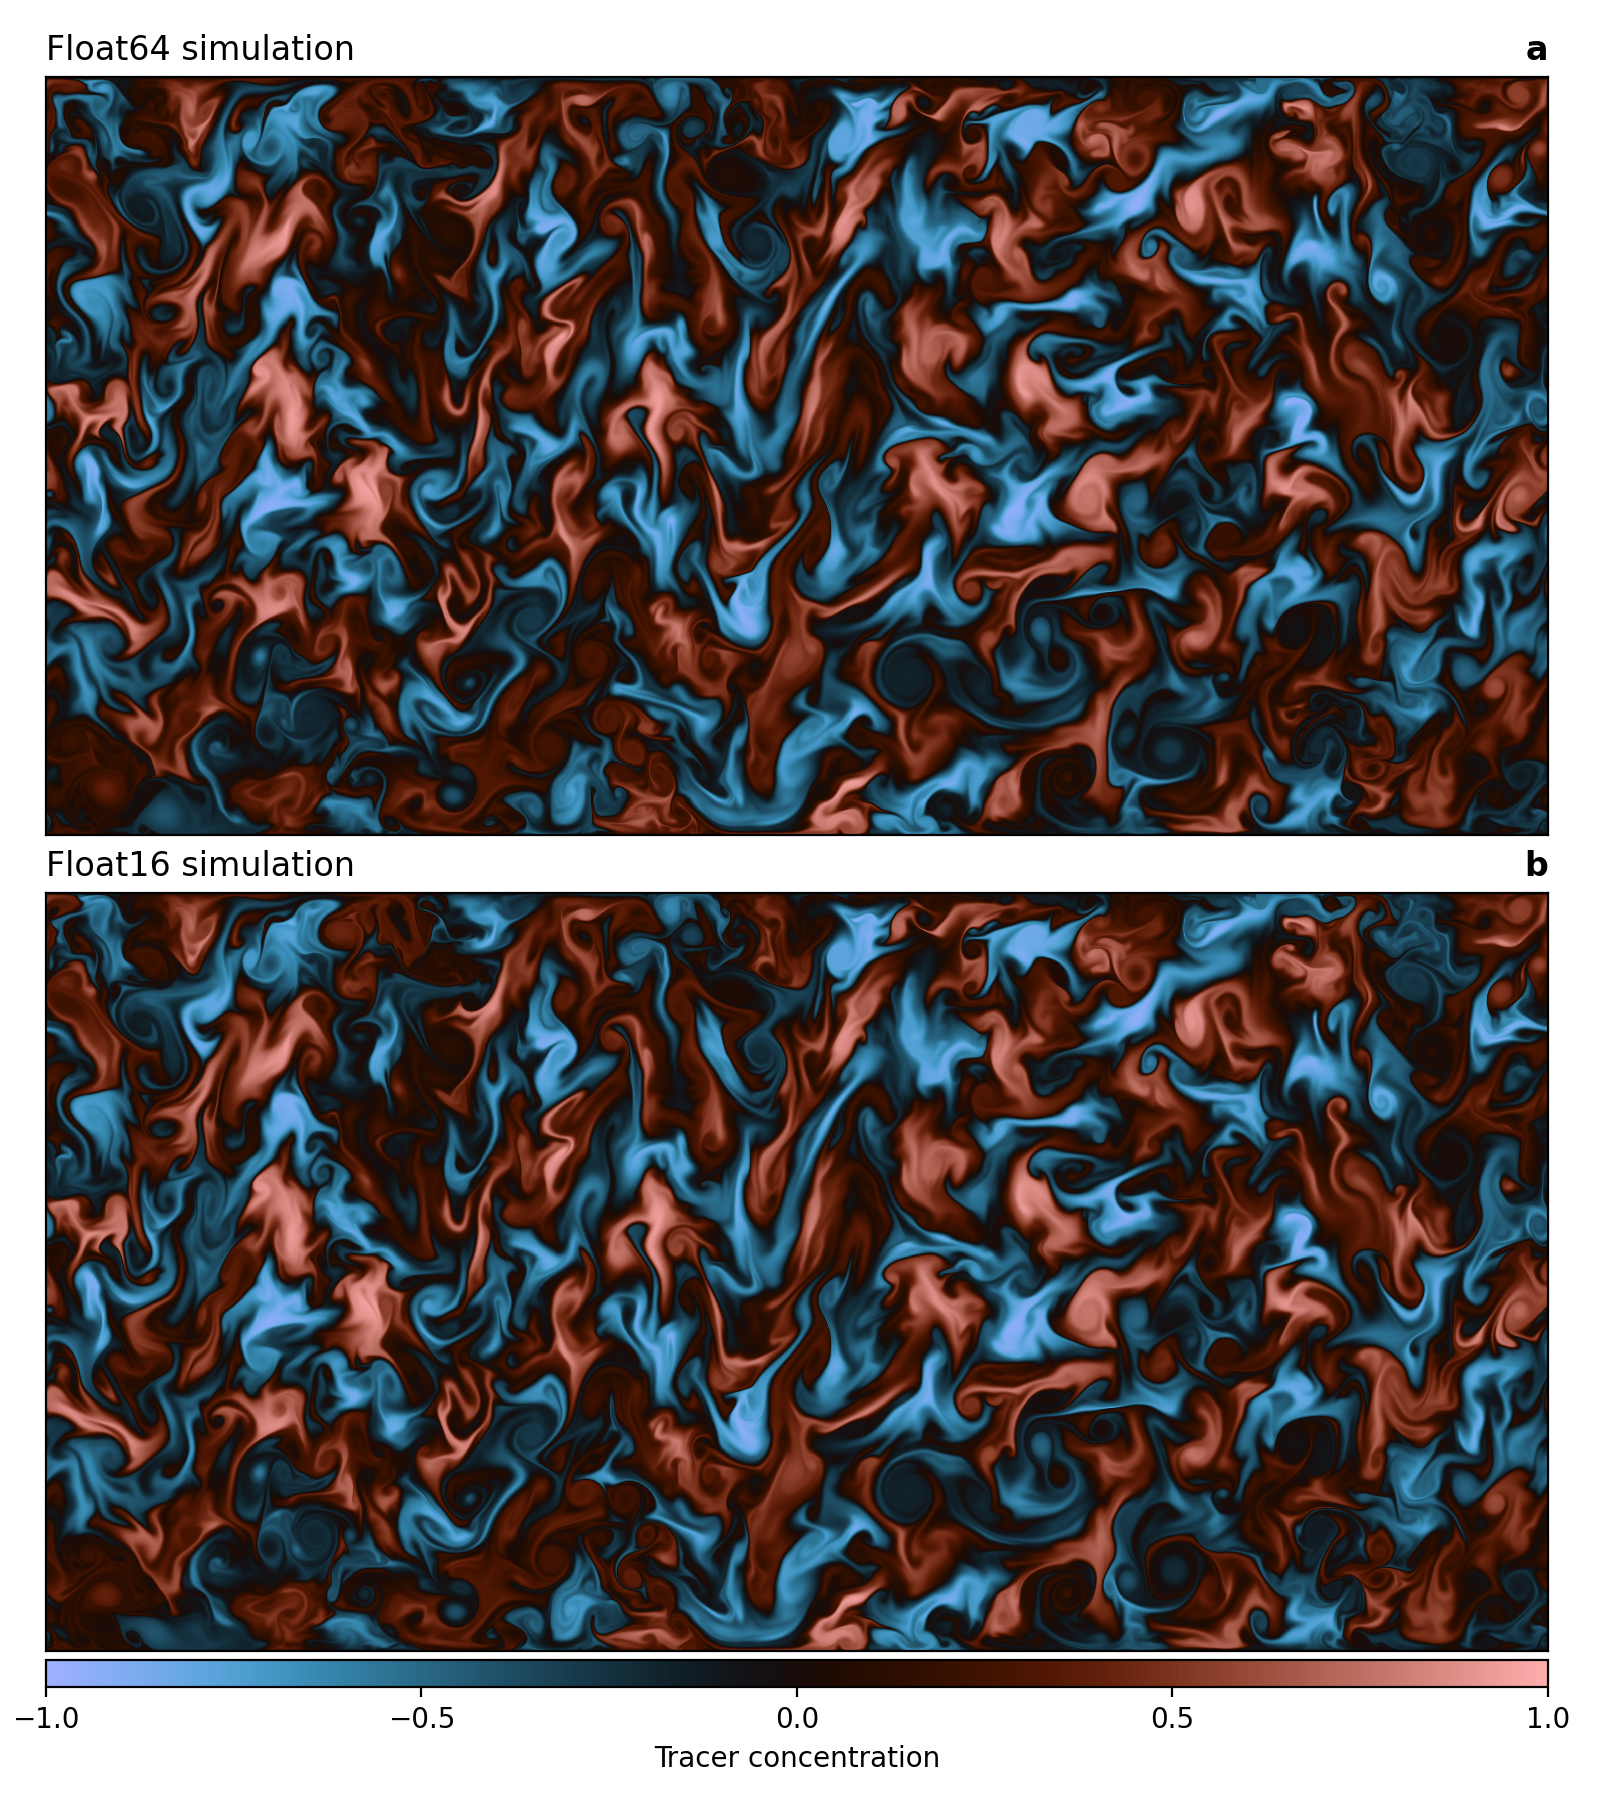
\includegraphics[width=1\textwidth]{Figures/a64fx/frame_hr_0199.png}
	\caption{\textbf{Turbulent tracer mixing as simulated by ShallowWaters.jl. a}
	Simulation based on Float64 arithmetic and \textbf{b} Float16 with compensated time integration.
	Snapshot is taken after 100 days of simulation (about 25,000 time steps) with 3000x1500 grid points
	starting from identical initial conditions. Remaining errors between \textbf{a} and \textbf{b} from
	low-precision Float16 are tolerable and will be masked by other sources of error in a less
	idealised model setup.}
	\label{fig:a64fx_tracermixing}
\end{figure}

Even after 100 days of simulation a large simulation (3000x1500 grid points) with Float16 shows minimal errors in
the tracer mixing compared to Float64 (Fig. \ref{fig:a64fx_tracermixing}). Only at regions near the boundaries,
where the mixing is enhanced, a difference is visible. The remaining rounding error is small and will be masked
in a more realistic setup by model or discretization errors. Reducing the precision in calculations raises concerns
about the numerical conservation of physically conserved quantities like mass. The compensated time integration
conserves the mass in the shallow water equations with Float16 (<0.002\% change within 500 days compared to Float64),
similar to mixed-precision (Fig. \ref{fig:a64fx_conservation}). Without compensated time integration for Float16 the conservation is with
0.05\% change over 500 days less accurate. Similar results were obtained for the conservation of the tracer.
We will now assess the speedups with Float16 compared to Float64 on A64FX.

\begin{figure}[tbhp]
	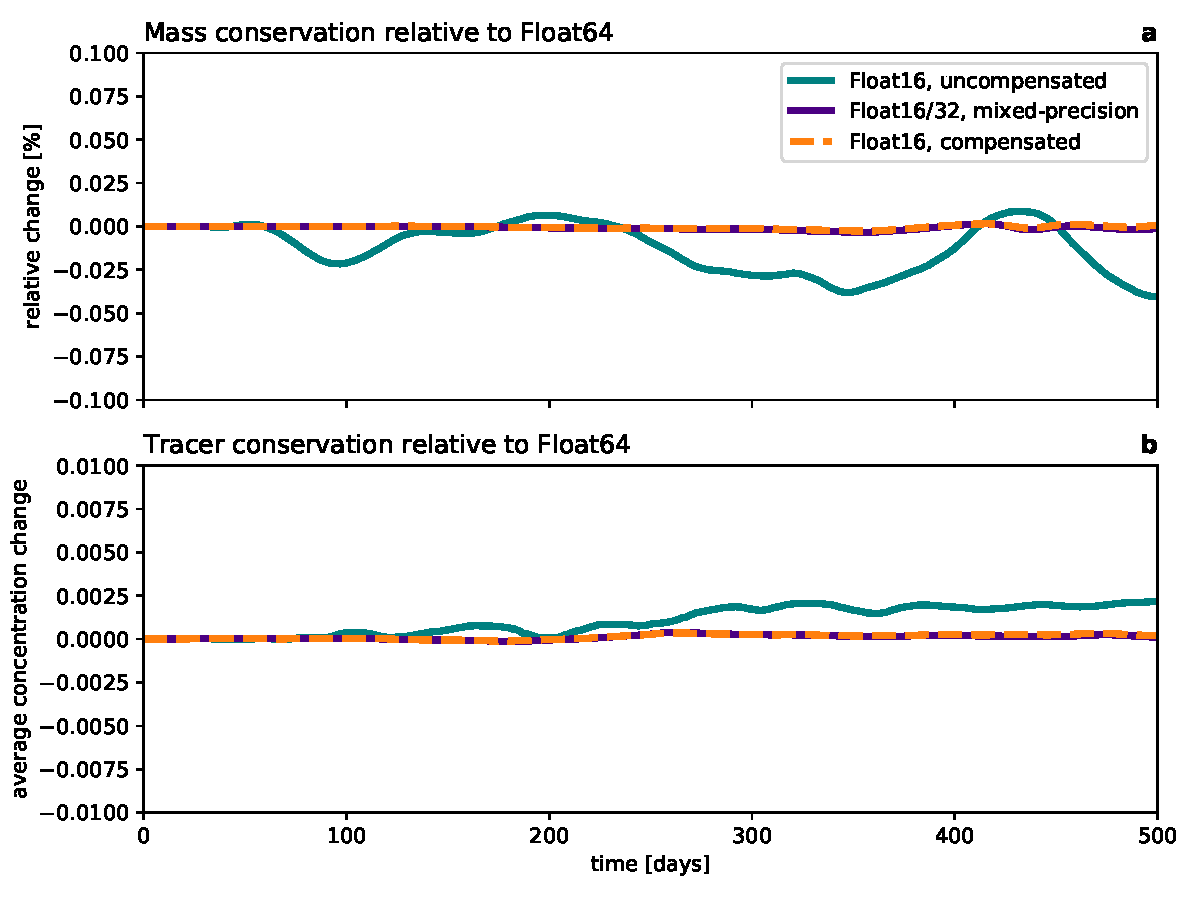
\includegraphics[width=1\textwidth]{Figures/a64fx/conservation.pdf}
	\caption{\textbf{Mass and tracer conservation with Float16 arithmetic. a}
	Mass conservation relative to Float64. \textbf{b} Tracer conservation relative to Float64 in units of tracer
	concentration with initial conditions in (-1,1), see Fig. \ref{fig:a64fx_tracermixing}. Both mass and tracer
	are well conserved with Float16 arithmetic. Best conservations are obtained with compensated time
	integration or mixed-precision.}
	\label{fig:a64fx_conservation}
\end{figure}

\subsection{Approaching 4x speedup on A64FX}
The A64FX is a microprocessor developed by Fujitsu based on the ARM-architecture. It powers not just the fastest
supercomputer in the world as of June 2021 (measured by TOP500.org, \cite{Dongarra2011}), Fugaku, but
also a number of smaller systems around the world, including Isambard 2 which we use here. The A64FX has a
number of features intended to accelerate machine learning applications. Notably, it allows not just Float32 and
Float64 arithmetic but also Float16. Official benchmarks of the A64FX demonstrate a cost increase which is linear
with the number of bits. In that sense, Float32 can be twice as fast in applications than Float64, while Float16 can
be four times as fast, when optimized well. In practice, speedups in complex applications are due to a mix of factors:
In compute-bound applications, the wall-clock time is largely given by the clock rate of the processor and the
vectorization of arithmetic operations (such that small sets of them are performed in parallel on a single processor core).
Using Float16 instead of Float64 allows to put four times as many numbers through the vectorization, theoretically
allowing for 4x speedups. The performance of memory-bound applications, on the other hand, is largely determined
by the data transfer rate between the processor and its various levels of caches that increase in size but decrease
in bandwidth. Using Float16 instead of Float64 allows to load four times as many numbers from memory,
which theoretically translates to 4x speedup as well. 

\begin{figure}[tbhp]
	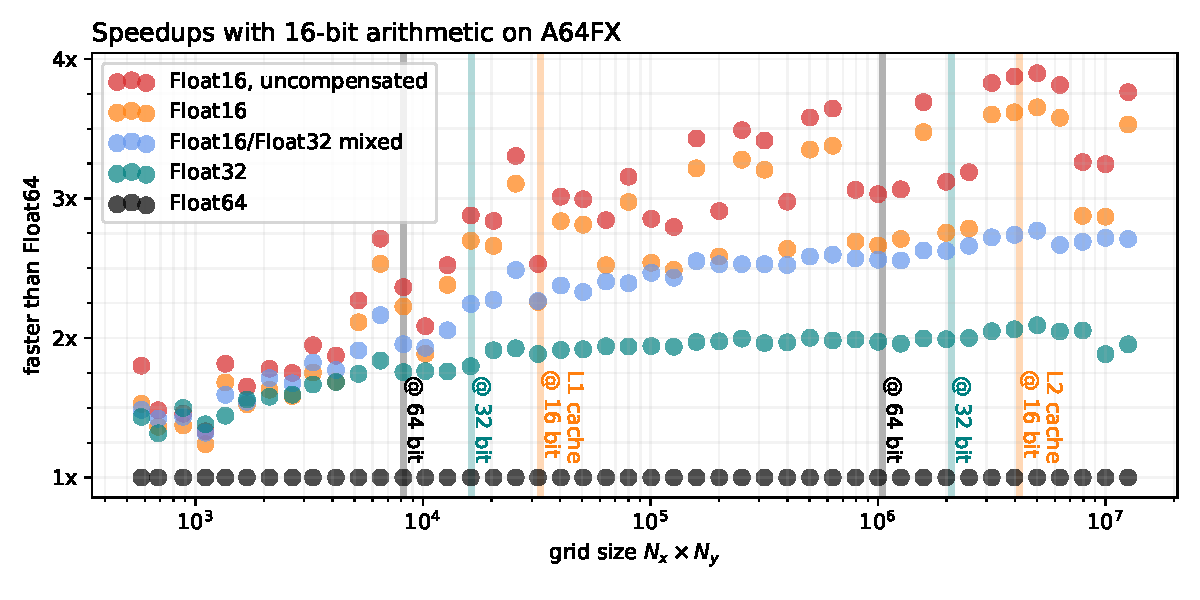
\includegraphics[width=1\textwidth]{Figures/a64fx/speedup.pdf}
	\caption{\textbf{Performance increase from Float16 when running ShallowWaters.jl at varying grid sizes
	on A64FX.} The grid size is the total number of grid points $N_x \times N_y$. All timings are single-threaded
	median wall clock times relative to Float64, excluding compilation, model initialisation and memory pre-allocation.
	The corresponding size of the L1 and L2 cache (64KiB, 8 MiB) of A64FX is given as vertical lines for arrays
	of 16, 32 and 64-bit floats.}
	\label{fig:a64fx_speedup}
\end{figure}

ShallowWaters.jl is a memory-bound application for which the biggest benefit from Float16 will be the reduction of
the size of the arrays by a factor of four when compared to Float64. The arrays can therefore be read faster from
memory with a potential speedup of 4x. We benchmark ShallowWaters.jl at varying grid sizes, excluding compilation,
model initialisation and memory pre-allocation. With grid sizes of $10^5$ (about 450x225 grid points) and larger,
there is a clear improvement from using Float32 instead of Float64 which approaches 2x speedups (Fig.
\ref{fig:a64fx_speedup}). Using Float16 these speedups reach up to 3.8x for grid sizes beyond $3 \cdot 10^6$
(about 2450x1225 grid points). The dependency of the speedup on the grid size is complicated:
While larger grids usually experience more acceleration on A64FX in Float16, there are ranges where the speedup
drops to 3-3.25x. This is likely due to peculiarities in the memory and cache hierarchy of the
A64FX, such that the performance benefit of Float16 cannot always be fully realised. A detailed assessment of these
peculiarities is beyond the scope of this study, but it is nevertheless reassuring that, even in the worst case, Float16
is still at least three times faster than Float64 for these large grids. 

As discussed in previous sections, using a compensated time integration can be used to minimize the rounding errors,
which comes with a small additional computational cost: Using the compensated time integration the speedups drop to
about 3.6x for large grids. Nevertheless, a compensated time integration yields higher performances than mixing the
precision of Float16 and Float32, which approaches only 2.75x here. Consequently, a compensated time integration
for Float16 is, although as precise, faster than mixed-precision.

\section{Discussion}
\label{sec:hardware_discussion}

Low-precision calculations for weather and climate simulations are a potential that is not yet fully exploited.
While the first weather forecast models are moving towards Float32, 16-bit arithmetics will likely find increasing
support on future supercomputers. We present, to our knowledge, the first fluid simulation that runs entirely in
hardware-accelerated 16 bit with minimal rounding errors but at almost 4x the speed. The simulations were
performed on A64FX, the microprocessor that is used in Fugaku, the fastest supercomputer as of November
2020 (TOP500, \cite{Dongarra2011}).

The complex partial differential equations underlying weather and climate simulations are difficult to fit into the
limited range of Float16, but here we have presented a method to do this more systematically. We present 
Sherlogs.jl to analyse number formats. Sherlogs.jl allows to assess any changes to the scaling of the equations
to minimise underflows while making the most of the available representable numbers. In our case,
subnormal floating-point numbers had to be avoided and scaling of the equations dropped the amount of
subnormals occurring below 0.2\%.

Using 16-bit floats will likely cause precision issues in fluid simulations. While mixed-precision has been
used to minimise rounding errors in precision-critical calculations, we have presented here an approach
that compensates for rounding errors to allow for simulations entirely within 16-bit arithmetic.
The compensated time integration minimises rounding errors from this precision-critical part of a simulation
at a slightly higher cost. Benchmarking in comparison to mixed-precision shows that the compensated
time integration is faster in ShallowWaters.jl while being as precise as mixed-precision.

Alternatives to floats have been discussed for weather and climate simulations previously \citep{Klower2019a,Klower2020a}.
Although posit numbers \citep{Gustafson2017a} are more precise in these applications, the improvement from floats to
posits is smaller than using mixed-precision and therefore also smaller than the compensated time integration.
In that sense, algorithms that are low-precision resilient are far more important than the actual choice of the
number format, especially given that only floats are widely hardware-supported.

The work here shows that a naive translation of the mathematical equations into code will likely fail with 16-bit arithmetic.
However, this does not mean that 16-bit arithmetic is unsuited for the numerical solution of complex partial differential
equations such as the shallow water equations. But it means that both precision and range issues have to be addressed
in the design of the algorithms used. A compensated time integration is a low-precision resilient algorithm,
and scaling is essential to fit the very limited range of Float16. 

While 16-bit hardware is largely designed for machine learning, its potential to increase computational efficiency
extends to weather and climate applications too. 16-bit calculations are indeed a competitive way to also accelerate
Earth-system simulations on available hardware.

